% Options for packages loaded elsewhere
\PassOptionsToPackage{unicode}{hyperref}
\PassOptionsToPackage{hyphens}{url}
%
\documentclass[
]{article}
\usepackage{lmodern}
\usepackage{amssymb,amsmath}
\usepackage{ifxetex,ifluatex}
\ifnum 0\ifxetex 1\fi\ifluatex 1\fi=0 % if pdftex
  \usepackage[T1]{fontenc}
  \usepackage[utf8]{inputenc}
  \usepackage{textcomp} % provide euro and other symbols
\else % if luatex or xetex
  \usepackage{unicode-math}
  \defaultfontfeatures{Scale=MatchLowercase}
  \defaultfontfeatures[\rmfamily]{Ligatures=TeX,Scale=1}
\fi
% Use upquote if available, for straight quotes in verbatim environments
\IfFileExists{upquote.sty}{\usepackage{upquote}}{}
\IfFileExists{microtype.sty}{% use microtype if available
  \usepackage[]{microtype}
  \UseMicrotypeSet[protrusion]{basicmath} % disable protrusion for tt fonts
}{}
\makeatletter
\@ifundefined{KOMAClassName}{% if non-KOMA class
  \IfFileExists{parskip.sty}{%
    \usepackage{parskip}
  }{% else
    \setlength{\parindent}{0pt}
    \setlength{\parskip}{6pt plus 2pt minus 1pt}}
}{% if KOMA class
  \KOMAoptions{parskip=half}}
\makeatother
\usepackage{xcolor}
\IfFileExists{xurl.sty}{\usepackage{xurl}}{} % add URL line breaks if available
\IfFileExists{bookmark.sty}{\usepackage{bookmark}}{\usepackage{hyperref}}
\hypersetup{
  pdftitle={Tecnicas y herramientas},
  hidelinks,
  pdfcreator={LaTeX via pandoc}}
\urlstyle{same} % disable monospaced font for URLs
\usepackage{graphicx}
\makeatletter
\def\maxwidth{\ifdim\Gin@nat@width>\linewidth\linewidth\else\Gin@nat@width\fi}
\def\maxheight{\ifdim\Gin@nat@height>\textheight\textheight\else\Gin@nat@height\fi}
\makeatother
% Scale images if necessary, so that they will not overflow the page
% margins by default, and it is still possible to overwrite the defaults
% using explicit options in \includegraphics[width, height, ...]{}
\setkeys{Gin}{width=\maxwidth,height=\maxheight,keepaspectratio}
% Set default figure placement to htbp
\makeatletter
\def\fps@figure{htbp}
\makeatother
\setlength{\emergencystretch}{3em} % prevent overfull lines
\providecommand{\tightlist}{%
  \setlength{\itemsep}{0pt}\setlength{\parskip}{0pt}}
\setcounter{secnumdepth}{-\maxdimen} % remove section numbering

\title{Tecnicas y herramientas}
\author{}
\date{}

\begin{document}
\maketitle

\hypertarget{metodologuxedas}{%
\section{Metodologías}\label{metodologuxedas}}

\hypertarget{scrum}{%
\subsection{Scrum}\label{scrum}}

Scrum es un marco de trabajo donde se ejecutan procesos ágiles que
contribuyen al desarrollo y mantenimiento de productos \emph{software}.
Por ello, está catalogado como una metodología ágil, la cual se
caracteriza por trabajar con un ciclo de vida iterativo e incremental,
donde se va liberando el producto \emph{software} de forma periódica a
través de {sprints} (iteraciones).

\hypertarget{cliente-de-control-de-versiones}{%
\section{Cliente de control de
versiones}\label{cliente-de-control-de-versiones}}

\begin{itemize}
\tightlist
\item
  Herramientas consideradas:
  \href{https://wiki.gnome.org/Apps/Gitg/}{Gitg},
  \href{https://www.syntevo.com/smartgit/}{Smartgit},
  \href{https://www.gitkraken.com/}{Gitkraken} y
  \href{https://desktop.github.com/}{GitHub Desktop}.
\item
  Herramienta elegida: \href{https://www.gitkraken.com/}{Gitkraken}.
\end{itemize}

GitKraken es un cliente para el control de versiones {Git} que nos
permite realizar todas y cada una de las tareas propias de {Git} a
través de una intuitiva y elegante interfaz gráfica. Además, incorpora
funciones adicionales como {GitFlow}, que nos permite gestionar las
diferentes ramificaciones del proyecto. De entre todas las opciones
posibles es, en mi opinión, la más competente tanto en diseño como en
funcionalidad.

\hypertarget{hosting-del-repositorio}{%
\section{\texorpdfstring{\emph{Hosting} del
repositorio}{Hosting del repositorio}}\label{hosting-del-repositorio}}

\begin{itemize}
\tightlist
\item
  Herramientas consideradas: \href{https://github.com/}{GitHub} y
  \href{https://gitlab.com/}{GitLab}.
\item
  Herramienta elegida: \href{https://github.com/}{GitHub}.
\end{itemize}

Github es el servicio de {hosting} de Git más utilizado para albergar
repositorios de código en la nube. El hecho de que cuente con una enorme
comunidad de usuarios y que además ofrezca servicios exclusivos y
gratuitos a estudiantes, lo convierte en la mejor opción posible. Alguno
de estos servicios son: repositorios privados, cantidad ilimitada de
colaboradores por repositorio y código propietario entre otros.

\hypertarget{gestor-de-contenidos}{%
\section{Gestor de contenidos}\label{gestor-de-contenidos}}

\begin{itemize}
\tightlist
\item
  Gestores de contenidos considerados:
  \href{https://duraspace.org/dspace/}{DSpace},
  \href{https://www.bibl.ulaval.ca/archimede/index.en.html}{Archimede},
  \href{https://www.mycore.de/}{MyCoRe},
  \href{https://omeka.org/classic/}{Omeka Classic},
  \href{https://github.com/geonetwork/core-geonetwork/}{Geonetwork} y
  \href{https://github.com/DANS-KNAW/dccd-webui}{DCCD}.
\item
  Gestor elegido: \href{https://omeka.org/classic/}{Omeka Classic}.
\end{itemize}

\emph{Omeka Classic} es una plataforma de gestión de contenido libre,
flexible y de código abierto. Su misión principal es la publicación de
colecciones digitales provenientes de bibliotecas, museos o cualquier
tipo de institución que pretenda difundir su patrimonio cultural, como
es el caso del CENIEH. Los motivos principales por los que se ha
decidido escoger esta aplicación son:

\begin{enumerate}
\def\labelenumi{\arabic{enumi}.}
\item
  Se distribuye bajo una Licencia Pública General (GNU), con lo cual su
  distribución, uso y modificación es libre.
\item
  Utiliza un entorno PHP-MySQL (Fácil despliegue sobre el servidor)
\item
  Basado en estándares internacionalmente aceptados como \emph{Dublin
  Core} o \emph{W3C}.
\item
  Flexible, escalable y extensible.

  \begin{quote}
  \begin{itemize}
  \tightlist
  \item
    \emph{Zend framework} como arquitectura.
  \item
    APIs documentadas.
  \item
    Le respalda una gran comunidad de usuarios y desarrolladores.
  \end{itemize}
  \end{quote}
\item
  Asistencia técnica gratuita gracias a la existencia de foros donde
  desarrolladores del proyecto oficial aportan soluciones.
\item
  Pensado para ser utilizado por usuarios no necesariamente expertos en
  el manejo de las TIC.
\end{enumerate}

\hypertarget{servidor-http-apache}{%
\section{Servidor HTTP Apache}\label{servidor-http-apache}}

El servidor \href{https://httpd.apache.org/}{HTTP Apache} es un servidor
web HTTP gratuito, de código abierto y multi-plataforma (Unix, Linux,
Windows y otras) que implementa el protocolo HTTP/1.1 y HTTP2. Alguna de
sus características más importantes son: su configuración e instalación
es bastante sencilla, puede ser extendido o adaptado a través de
módulos, incorpora funciones para la autentificación y validación de
usuarios, y da soporte a varios lenguajes de programación como PHP y
Python.

\hypertarget{mysql}{%
\section{MySQL}\label{mysql}}

\href{https://www.mysql.com/}{MySQL} es uno de los sistemas de gestión
de base de datos más utilizados en la actualidad. Gestiona bases de
datos relacionales, es decir, aquellas que siguen el modelo relacional.
Es gratuito, multi-plataforma (disponible en Linux, Windows y Unix) y es
utilizado con numerosos lenguajes de programación, siendo el más
utilizado con diferencia PHP.

\hypertarget{libreruxedas}{%
\section{Librerías}\label{libreruxedas}}

\hypertarget{zend-framework}{%
\subsection{\texorpdfstring{\emph{Zend
Framework}}{Zend Framework}}\label{zend-framework}}

\href{https://framework.zend.com/}{Zend Framework} (ZF) es un
\emph{framework} de PHP desarrollado por la compañia \emph{Zend
Technologies}, principal responsable del mantenimiento del lenguaje de
programación PHP. A través de ZF se pueden desarrollar aplicaciones web
de una forma mucho más rápida y sencilla que utilizando PHP puro. Como
características más destacables, aporta componentes que se pueden
reutilizar en el código base de la aplicación, emplea el patrón de
diseño MVP, con las ventajas que eso conlleva, y permite escalar la
aplicación web con el concepto de módulos (\emph{plugins}).

\hypertarget{phpunit}{%
\subsection{\texorpdfstring{\emph{PHPUnit}}{PHPUnit}}\label{phpunit}}

\href{https://phpunit.de/}{PHPUnit} es un \emph{framework} utilizado
para desarrollar pruebas unitarias sobre aplicaciones basadas en PHP. Es
un proyecto \emph{open-source} creado por Sebastian Bergmann cuyo
repositorio oficial se encuentra en
\href{https://github.com/sebastianbergmann/phpunit}{Github}.

\hypertarget{zipstream}{%
\subsection{\texorpdfstring{\emph{ZipStream}}{ZipStream}}\label{zipstream}}

\href{https://github.com/maennchen/ZipStream-PHP/tree/0.2.2}{ZipStream}
es una librería de PHP que permite transmitir archivos zip de forma
dinámica, sin necesidad de ocupar espacio en el servidor.

\hypertarget{leaflet}{%
\subsection{\texorpdfstring{\emph{Leaflet}}{Leaflet}}\label{leaflet}}

\href{https://github.com/Leaflet/Leaflet}{Leaflet} es una librería
\emph{open-source} de \emph{JavaScript} utilizada para crear mapas
interactivos sobre aplicaciones web. Sorprende lo ligera que es (39kB)
para la cantidad de servicios que ofrece. Además de las funciones
presentes en su versión original, se pueden añadir nuevas funciones
gracias a los \emph{plugins} desarrollados por la comunidad.

\hypertarget{leaflet-draw}{%
\subsubsection{\texorpdfstring{\emph{Leaflet
draw}}{Leaflet draw}}\label{leaflet-draw}}

\href{https://github.com/Leaflet/Leaflet.draw}{Leaflet draw} es una
extensión de la librería \emph{Leaflet} que provee herramientas para
dibujar y editar figuras sobre los mapas creados por esta librería.
Permite delimitar regiones con múltiples formas (rectangular, circular,
etc.), bastante útil cuando el marcador por defecto no es suficiente
para señalar una determinada ubicación.

\hypertarget{jquery}{%
\subsection{\texorpdfstring{\emph{jQuery}}{jQuery}}\label{jquery}}

\href{https://jquery.com/}{jQuery} es una de las librerías más conocidas
de \emph{Javascript}. Aporta multitud de funciones que facilitan el
desarrollo de aplicaciones web enriquecidas del lado del cliente. Estas
permiten llevar a cabo servicios tales como la manipulación de
documentos HTML, el manejo de eventos, animaciones, ajax, etc.

\hypertarget{notify}{%
\subsubsection{\texorpdfstring{\emph{Notify}}{Notify}}\label{notify}}

\href{https://notifyjs.jpillora.com/}{Notify} es una extensión de la
librería \emph{jQuery} que proporciona notificaciones simples altamente
personalizables. Es un buen medio para mantener informado al usuario
ante determinadas acciones o eventos.

\hypertarget{sweet-alert-2}{%
\subsubsection{\texorpdfstring{\emph{Sweet alert
2}}{Sweet alert 2}}\label{sweet-alert-2}}

\href{https://github.com/sweetalert2/sweetalert2}{Sweet alert 2} es una
extensión de la librería \emph{jQuery} que permite crear \emph{popups}
(ventanas emergentes) de alerta personalizados. Es una buena alternativa
a los \emph{popups} de alerta que Javascript ofrece por defecto ya que
se pueden añadir nuevas funciones que mejores la calidad de información
mostrada al cliente.

\hypertarget{patruxf3n-de-diseuxf1o}{%
\section{Patrón de diseño}\label{patruxf3n-de-diseuxf1o}}

\hypertarget{mvp-modelo-vista-controlador}{%
\subsection{MVP
(Modelo-Vista-Controlador)}\label{mvp-modelo-vista-controlador}}

MVP es un patrón de diseño muy utilizado en el desarrollo de
aplicaciones web. Permite organizar el código en tres secciones
diferentes: Modelo, Vista y Controlador. La primera se encarga del
manejo de los datos y la lógica de negocio, la segunda está relacionada
con el diseño y la presentación, y la tercera interactúa con las dos
primeras.

\begin{figure}
\hypertarget{mvc}{%
\centering
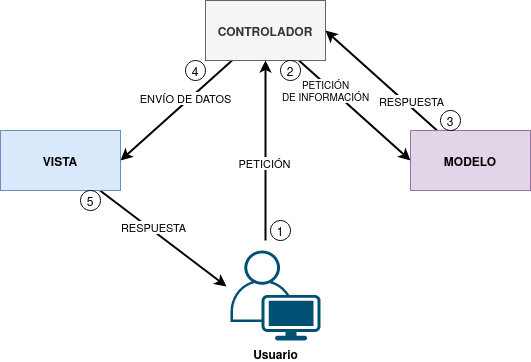
\includegraphics{../_static/images/mvc.png}
\caption{Diagrama que muestra la relación entre Modelo, Vista y
Controlador}\label{mvc}
}
\end{figure}

\begin{itemize}
\tightlist
\item
  \textbf{Modelo}: modifica, gestiona y actualiza los datos de la
  aplicación. En el caso de contar con una única base de datos, sería la
  capa donde se encuentra el código relacionado con las consultas,
  búsquedas, filtros y actualizaciones.
\item
  \textbf{Vista}: muestra al usuario final la interfaz gráfica de la
  aplicación, es decir, las páginas, ventanas, formularios, etc. En
  términos de programación se correspondería con el \emph{frontend}.
\item
  \textbf{Controlador}: gestiona, atiende y procesa las peticiones
  realizadas por parte de los usuarios. A través de esta capa se
  comunican el modelo y la vista. Como vemos en la \texttt{mvc}, el
  controlador solicita los datos necesarios al modelo, se manipulan
  acorde a la petición del usuario y se entregan a la vista de forma que
  el usuario pueda visualizar los resultados esperados.
\end{itemize}

\hypertarget{entorno-de-desarrollo-integrado-ide}{%
\section{Entorno de desarrollo integrado
(IDE)}\label{entorno-de-desarrollo-integrado-ide}}

\hypertarget{php-css-javascript-xml}{%
\subsection{\texorpdfstring{\emph{PHP} \textbar{} \emph{CSS} \textbar{}
\emph{JavaScript} \textbar{}
\emph{XML}}{PHP \textbar{} CSS \textbar{} JavaScript \textbar{} XML}}\label{php-css-javascript-xml}}

\begin{itemize}
\tightlist
\item
  Herramientas consideradas: \href{https://netbeans.org/}{NetBeans},
  \href{https://atom.io/}{Atom}, \href{https://eclipse.org/}{Eclipse},
  \href{https://www.zend.com/products/zend-studio}{Zend Studio} y
  \href{https://www.activestate.com/products/komodo-ide/}{Komodo}.
\item
  Herramienta elegida: \href{https://netbeans.org/}{NetBeans}.
\end{itemize}

NetBeans es un entorno de desarrollo muy completo escrito en Java.
Contiene una gran cantidad de funcionalidades y da soporte a todos y
cada uno de los lenguajes de programación utilizados en el desarrollo de
la infraestructura \emph{software}. Además, se pueden instalar
complementos que permiten extender su compatibilidad con otros marcos de
trabajo como \emph{Zend Framework}.

\hypertarget{latex}{%
\subsection{LaTeX}\label{latex}}

\begin{itemize}
\tightlist
\item
  Herramientas consideradas:
  \href{https://www.texstudio.org/}{TeXstudio} y
  \href{http://www.xm1math.net/texmaker/}{Texmaker}.
\item
  Herramienta elegida:
  \href{http://www.xm1math.net/texmaker/}{Texmaker}.
\end{itemize}

\emph{Texmaker} es un editor libre y gratuito para LaTeX distribuido
bajo la licencia GPL. Incluye múltiples herramientas necesarias para
elaborar documentos tanto con LaTeX como BibText o Metapost. También
incorpora funciones adicionales como la corrección ortográfica, el
auto-completado y plegado de código o un visor de pdf compatible con
SyncTeX y con modo de visualización continua. Además, es
multi-plataforma, disponible tanto en UNIX como en MacOS y Windows.

\hypertarget{generador-de-documentaciuxf3n}{%
\section{Generador de
documentación}\label{generador-de-documentaciuxf3n}}

\begin{itemize}
\tightlist
\item
  Herramientas consideradas:
  \href{https://www.sphinx-doc.org/es/master/index.html}{Sphinx} y
  \href{https://www.mkdocs.org/}{Mkdocs}.
\item
  Herramienta elegida:
  \href{https://www.sphinx-doc.org/es/master/index.html}{Sphinx}.
\end{itemize}

He decidido utilizar el generador de documentación \emph{Sphinx} ya que
es mucho más completo que \emph{MkDocs}. Además de soportar el lenguaje
de marcado ligero \emph{Markdown} es compatible con
\emph{reStructuredText}. Esta compatibilidad hace que sea posible usar
ambos lenguajes en un mismo proyecto \emph{Sphinx}. Además, con el uso
del conversor \href{http://pandoc.org/}{Pandoc}, toda la documentación
generada a partir de ambos lenguajes se puede exportar a multitud de
formatos, entre los que se encuentra LaTeX.

\emph{Markdown} es un lenguaje muy conocido debido a que es utilizado en
plataformas como \emph{Github} o \emph{StackOverflow}. Fue creado para
generar contenido de una manera sencilla de escribir y fácil de leer.
Permite además convertir el texto marcado en documentos \emph{XHTML}.

\emph{reStructuredText} presenta también una sintaxis sencilla y de
fácil lectura. La principal ventaja respecto a \emph{Markdown} es que
permite elaborar expresiones más complejas sin el uso de
librerías/aplicaciones externas.

\emph{LaTeX} es el estándar de facto para la publicación de documentos
científicos. Permite la creación de documentos con una alta calidad
tipográfica. Utiliza \emph{Tex} como motor a la hora de darle formato a
los documentos.

\hypertarget{herramientas-de-integraciuxf3n-continua}{%
\section{Herramientas de integración
continua}\label{herramientas-de-integraciuxf3n-continua}}

\hypertarget{compilaciuxf3n-y-despliegue}{%
\subsection{Compilación y
Despliegue}\label{compilaciuxf3n-y-despliegue}}

\begin{itemize}
\tightlist
\item
  Herramientas consideradas:
  \href{https://github.com/features/actions}{Github Actions},
  \href{https://travis-ci.org/}{Travis CI} y
  \href{https://jenkins.io/}{Jenkins}.
\item
  Herramienta elegida: \href{https://github.com/features/actions}{Github
  Actions}.
\end{itemize}

Para aplicar la integración continua al proyecto se ha dedicido utilizar
\emph{Github Actions}. El principal motivo de esta elección es que todas
sus funciones se encuentran integradas en la propia interfaz de
\emph{Github}, lo que facilita en gran medida su uso. Además, permite
reutilizar código elaborado por otros usuarios de la comunidad en los
flujos de trabajo (\emph{workflows}) personales.

\hypertarget{calidad-del-cuxf3digo}{%
\subsection{Calidad del código}\label{calidad-del-cuxf3digo}}

\begin{itemize}
\tightlist
\item
  Herramientas consideradas: \href{https://codacy.com}{Codacy},
  \href{https://codecov.io/}{Codecov} y
  \href{https://codeclimate.com/}{CodeClimate}.
\item
  Herramienta elegida: \href{https://codacy.com}{Codacy}.
\end{itemize}

La opción escogida ha sido \emph{Codacy} ya que, de entre las tres
propuestas, es la que está más enfocada a la revisión de código
automatizada, que es lo se estaba buscando. Da soporte a todos los
lenguajes que se han utilizado en el proyecto ( \emph{PHP}, \emph{HTML},
\emph{JavaScript} y \emph{CSS} ). Además, el proceso de configuración no
se hace nada pesado gracias a que se puede llevar a cabo desde su propia
interfaz gráfica. Entre sus configuraciones más utilizadas están la
exclusión de ficheros, la activación/desactivación de patrones de
código, la selección de ramas y la gestión de integraciones.

\hypertarget{documentaciuxf3n-continua}{%
\subsection{Documentación continua}\label{documentaciuxf3n-continua}}

\href{https://readthedocs.org/}{Read the Docs} es una plataforma web que
facilita la tarea de documentar productos \emph{software} automatizando
la compilación, versionado y hospedaje de los ficheros generados por la
herramienta de documentación \emph{Sphinx}. El proceso es muy sencillo,
basta con alojar la documentación \emph{Sphinx} en un repositorio,
realizar un \emph{commit} sobre este y, automáticamente, se actualizan
los cambios en la documentación alojada en \emph{readthedocs.org}.
Presenta múltiples formatos de exportación y permite configurar
múltiples aspectos (traducciones, variables de entorno, reglas de
automatización, etc.). Todos estos servicios se ofrecen de forma
gratuita.

\hypertarget{herramienta-de-diagramaciuxf3n}{%
\section{Herramienta de
diagramación}\label{herramienta-de-diagramaciuxf3n}}

\begin{itemize}
\tightlist
\item
  Herramientas consideradas:
  \href{https://es.libreoffice.org/descubre/draw/}{Draw - LIbreOffice},
  \href{https://www.smartdraw.com/}{SmartDraw} y
  \href{https://app.diagrams.net/}{Draw.io}.
\item
  Herramienta elegida: \href{https://app.diagrams.net/}{Draw.io}.
\end{itemize}

\emph{Draw.io} es una herramienta gratuita de diseño que permite crear y
compartir diagramas \emph{on-line}, es decir, sin necesidad de instalar
programa alguno. Presenta una interfaz elegante y fácil de utilizar
desde la cual podemos hacer uso de sus múltiples funciones como, por
ejemplo, importar imágenes, añadir objetos UML, exportar e importar
proyectos en diversos formatos, etc.

\hypertarget{herramientas-de-comunicaciuxf3n}{%
\section{Herramientas de
comunicación}\label{herramientas-de-comunicaciuxf3n}}

\hypertarget{microsoft-teams}{%
\subsection{\texorpdfstring{\emph{Microsoft
Teams}}{Microsoft Teams}}\label{microsoft-teams}}

A través de
\href{https://www.microsoft.com/es-es/education/products/teams}{Microsoft
Teams} se han llevado a cado las reuniones de cada \emph{sprint}.
\emph{Teams} viene integrado en el paquete de \emph{Microsoft Office
365}, por lo que es un servicio que puede ser adquirido por el personal
de la UBU. Ofrece una gran cantidad de funcionalidades relacionadas con
la comunicación como, por ejemplo, la creación de chats personalizados
(individuales/grupales, públicos/privados, etc.), compartición de
pantalla, integración de aplicaciones externas (Stream, Excel, etc.) o
introducción de efectos de cámara (efectos de fondo, filtros, etc.).

\hypertarget{zoom}{%
\subsection{\texorpdfstring{\emph{Zoom}}{Zoom}}\label{zoom}}

{Zoom \textless https://zoom.us/\textgreater{}} es la herramienta de
comunicación con la que se han llevado a cabo las reuniones tanto con el
CENIEH como con ARIADNEplus. Al igual que la herramienta \emph{Microsoft
Teams}, permite realizar videollamadas y reuniones virtuales con
multitud de funcionalidades extra.

\hypertarget{otras-herramientas}{%
\section{Otras herramientas}\label{otras-herramientas}}

\hypertarget{docker}{%
\subsection{\texorpdfstring{\emph{Docker}}{Docker}}\label{docker}}

La tecnología \href{https://www.docker.com/}{Docker} permite desplegar
una aplicación distribuida y empaquetarla junto a todas sus dependencias
y librerías en un uno o varios "objetos" denominados contenedores o
\emph{containers}. Estos pueden ser ejecutados en cualquier servidor
Linux, aumentando así la flexibilidad y portabilidad de nuestra
aplicación.

\hypertarget{google-cloud}{%
\subsection{\texorpdfstring{\emph{Google
Cloud}}{Google Cloud}}\label{google-cloud}}

\href{https://cloud.google.com/}{Google Cloud} es una plataforma creada
por la compañía \emph{Google} desde la que puedes acceder a numerosos
servicios relacionados con el desarrollo web. Alguno de sus servicios
son: \emph{Cloud Computing}, \emph{Networking}, \emph{Data Storage},
\emph{Data Analytics}, \emph{Machine learning}, etc.

\hypertarget{gke-google-kubernetes-engine}{%
\subsubsection{\texorpdfstring{\emph{GKE -- Google Kubernetes
Engine}}{GKE -- Google Kubernetes Engine}}\label{gke-google-kubernetes-engine}}

\href{https://cloud.google.com/kubernetes-engine}{Google Kubernetes
Engine} (GKE) proporciona un entorno desde donde puedes implementar,
administrar y escalar aplicaciones en contenedores mediante la
infraestructura de \emph{Google}. El entorno de GKE consta de varias
máquinas (en particular, instancias de \emph{Compute Engine}) que se
agrupan para formar un clúster.

\hypertarget{kubernetes}{%
\subsection{\texorpdfstring{\emph{Kubernetes}}{Kubernetes}}\label{kubernetes}}

\href{https://kubernetes.io/es/}{Kubernetes} es una plataforma
\emph{open-source} que permite automatizar los procesos relacionados con
la implementación, administración y escalabilidad de contenedores. He
decidido utilizar este orquestador (\emph{orchestrator}) para desplegar
mi aplicación en la nube (\emph{Google Cloud}) por la gran cantidad de
ventajas que ofrece como, por ejemplo, autoreparación de contenedores,
utilización de \emph{secrets} o despliegues y rollbacks automáticos.

\hypertarget{kustomize}{%
\subsection{\texorpdfstring{\emph{Kustomize}}{Kustomize}}\label{kustomize}}

\href{https://github.com/kubernetes-sigs/kustomize}{Kustomize} es una
herramienta que permite operar sobre objetos de la plataforma
\emph{Kubernetes} a través de un archivo de personalización.

\end{document}
